\chapter{LITERATURE REVIEW}

% \section{Service Robot}

\section{Elderly}
Elderly refers to individuals who are around 65 years of age or older. Socially, people categorized as elderly are those who are 65 years or older and may require medicare or home health services. According to the United Nations (UN), an individual is classified as elderly or an older person when they reach the age of 60 or older. The increasing number of elderly individuals is considered one of the four megatrends that can affect sustainable development \cite{nations2019world}.

% Elderly merujuk kepada individu yang memiliki sekitar 65 tahun atau lebih. Secara sosial, orang-orang yang dikategorikan sebagai elderly adalah individu yang memiliki usia 65 tahun atau lebih yang membutuhkan mediacare atau layanan kesehatan di rumah. Menurut United Nation (UN), seseorang dikategorikan sebagai elderly atau older person ketika seseorang telah mencapai usia 60 tahun lebih. Jumlah elderly yang semakin bertambah ini telah dianggap sebagai salah satu dari empat megatrends yang dapat mempengaruhi pembangunan berkelanjutan \cite{nations2019world}.

\begin{figure}[H]
    \centering
    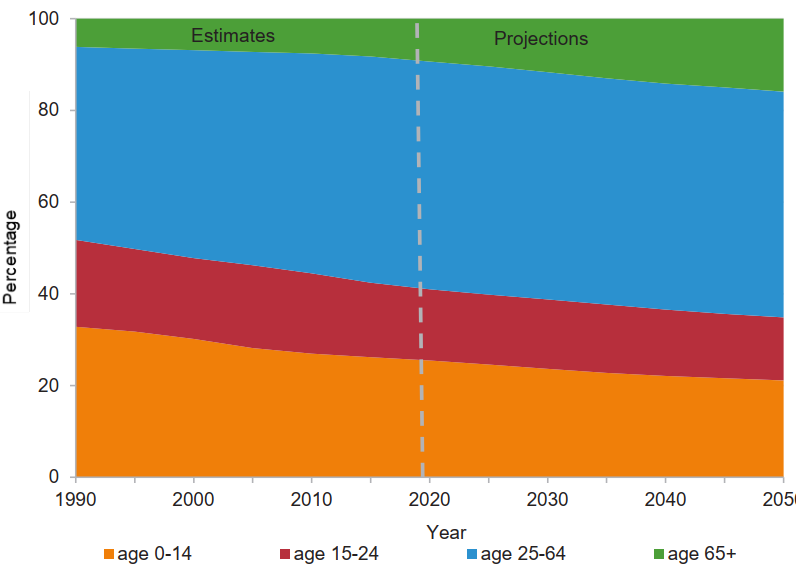
\includegraphics[width=0.75\textwidth]{bab2/ar_PopulationbyAge.png}
    \caption{Global population by age distribution.}
    \label{fig:PopulationbyAge}
\end{figure}

The global population of elderly individuals has been growing rapidly. This trend is predicted to continue growing significantly in the future. According to data from the United Nations (UN) in 2019, the global number of elderly people aged 65 years or older reached 703 million (9\% of the total global population). This number is projected to continue rising and double in the next three decades, which means 2050. Fig. \ref{fig:PopulationbyAge} illustrates the distribution of the global population categorized by age groups. The elderly population is expected to continue growing as the decline in the working-age population decreases.

% Populasi elderly di dunia telah meningkat secara pesat. Tren ini akan diprediksi terus bertambah banyak kedepannya. Berdasarkan data dari UN pada tahun 2019, jumlah elderly secara global telah mencapai jumlah 703 juta orang berusia 65 tahun atau lebih. Jumlah ini diproyeksikan akan terus meningkat dan menjadi dua kali lipatnya tiga dekade kedepan atau pada tahun 2050. Fig. \ref{fig:PopulationbyAge} menunjukkan pesebaran populasi global yang dibedakan berdasarkan rentang usia. Elderly diproteksikan akan terus bertambah seiring pengurangan penurunan masyarakat usia produktif.

As individuals age, they are highly likely to experience various physical and mental changes and conditions, such as decreased mobility, loss of sensory functions, depression, difficulty expressing themselves, and a decline in physical abilities. In some cases, the elderly require assistance in performing daily activities. Accompanying and providing support to the elderly has become a dedicated focus for researchers. Solving the issues related to the safety and daily care of the elderly requires research proposals in activity recognition \cite{elderly1}.

% Seiring bertambahnya usia, seseorang sangat mungkin mengalami kondisi dan perubahan pada dirinya baik secara fisik maupun mental, seperti penurunan mobilitas, hilangnya fungsi indera tubuh, depresi, kurangnya dalam mengekspresikan diri, hingga penurunan kemampuan fisik. Dalam beberapa kasus, elderly membutuhkan bantuan dalam menjalankan beberapa kegiatannya. Pendampingan terhadap elderly telah menjadi konsentrasi tersendiri bagi para peneliti. Penyelesaian masalah mengenai keamanan perawatan dan sehari-hari elderly membutuhkan usulan riset dalam pengenalan aktifitasnya \cite{elderly1}.

\section{Elderly Physical Issue}
\label{sec2:ElderlyPhysicalIssue}

The issue of eldelry health has become important since the increase in the number of elderly in the world. Increasing age makes the elderly experience a decrease in organ or tissue function. Diseases that affect the elderly can vary, such as chronic health problems, mobility and balance, decreased sensory function, and physical issues. For physical issues, diseases affect the muscles and bones of the elderly. Strengthening these body parts is important because they are the main support of the body \cite{PhysicalIssue}. Some of the physical issues that affect the elderly are explained in this section.

\subsection{Frozen Shoulder and Exercise Activity}
\label{subsec2:FrozenShoulder}

\begin{figure}[h!]
    \centering
    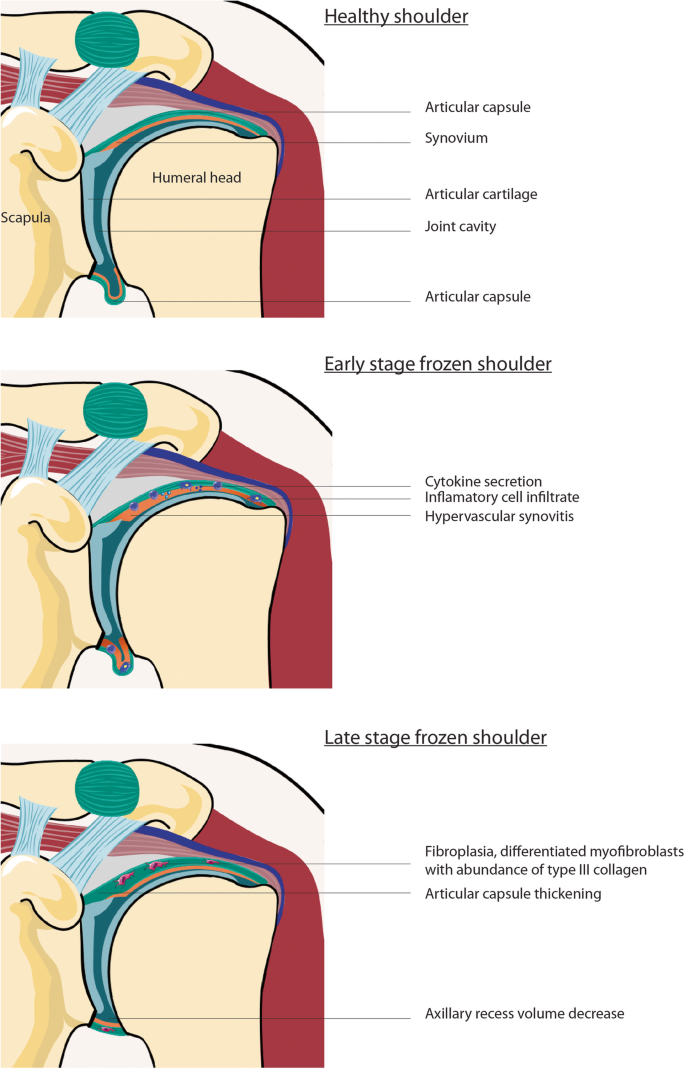
\includegraphics[width=0.75\textwidth]{bab2/ar_FrozenShoulder.png}
    \caption{Comparison of healthy shoulders with those with frozen shoulder \cite{FrozShoulder4}.}
    \label{fig:FrozenShoulder}
\end{figure}

Frozen shoulder, another name for adhesive capsulitis, is a common shoulder condition marked by a progressive rise in pain and stiffness. Women are more likely than males to be impacted, and it usually affects those over 40. The illness develops in three stages: freezing (painful), adhering, and melting. It usually goes away on its own in one to three years \cite{FrozenShoulder2}. There are two categories of frozen shoulder: primary and secondary. Primary frozen shoulder is caused by the presence of pericapsular attachments, while secondary frozen shoulder is caused by various factors such as sprains, strains, tendinopathy, tendon tears, or bursitis \cite{FrozenShoulder1}.

In the frozen period, strengthening activities such isometric shoulder external rotation, posterior capsule stretch, and scapular retraction might be introduced. Stretching and strengthening exercises can also get more intense during the thawing phase by holding onto the poses for longer periods of time.

Case studies demonstrate how well physical therapy works to improve joint mobility and day-to-day functioning. For instance, a case study published in the Journal of the Formosan Medical Association described how physiotherapy was used to treat a patient with primary frozen shoulder, leading to better joint mobility and ability to do everyday tasks.

These physical issues can be prevented using exercise activities. A wide variety of exercise activities can prevent these physical issues. Exercise activities that move the shoulder are the main focus of the movement. Some of the training activities are shoulder flexion extension \cite{ShoulderFlexionExtension}, adduction abduction \cite{AdductionAbduction}, and arm circumduction \cite{ArmCircumduction}.
% Isu fisik ini dapat dicegah menggunakan aktifitas latihan. Berbagai macam aktifitas latihan mampu mencegah munculnya isu fisik ini. Aktifitas latihan yang menggerakkan bagian bahu menjadi fokus utama pada gerakannya. Beberapa aktifitas latihan adalah shoulder flxion extension \cite{ShoulderFlexionExtension}, adduction abduction \cite{AdductionAbduction}, dan arm circumduction \cite{ArmCircumduction}.

Shoulder flexion and extension are the two main types of movements performed by the shoulder joint, which involve moving the arm around the body axis. Shoulder flexion is the movement of raising the arm forwards and upwards, away from the body. It involves muscles such as the anterior deltoid, pectoralis major and coracobrachialis. An example of this movement is when an individual lifts the arm straight forward until the arm is above the head. Shoulder extension is the movement of moving the arm behind the body. This movement involves muscles such as the posterior deltoid, latissimus dorsi, and teres major. An example of this movement is when individuals swing their arms backwards while walking or running \cite{ShoulderFlexionExtension1}.
% Shoulder flexion dan extension adalah dua jenis gerakan utama yang dilakukan oleh sendi bahu, yang melibatkan pergerakan lengan di sekitar sumbu tubuh. Shoulder flexion adalah gerakan mengangkat lengan ke depan dan ke atas, menjauh dari tubuh. Gerakan ini melibatkan otot-otot seperti deltoid anterior, pectoralis major, dan coracobrachialis. Contoh dari gerakan ini adalah ketika individu mengangkat lengan lurus ke depan hingga lengan berada di atas kepala. Shoulder extension adalah gerakan menggerakkan lengan ke belakang tubuh. Gerakan ini melibatkan otot-otot seperti deltoid posterior, latissimus dorsi, dan teres major. Contoh dari gerakan ini adalah ketika individu mengayunkan lengan ke belakang saat berjalan atau berlari \cite{ShoulderFlexionExtension1}.

Adduction and abduction arm movements are two types of movements that involve the displacement of the arm with respect to the body axis. Adduction is the movement of bringing the arm closer towards the centerline of the body. When the arm moves from a distant position towards the body is called adduction. For example, when an individual brings the arm to the side of the body. While abduction is the movement of moving the arm away from the midline of the body. When the arm moves from a position near the body outwards it is called abduction. For example, when individuals raise their arms to the side away from the body. These two movements in a series are often used in various physical activities and exercises to train certain muscles and increase flexibility and body strength \cite{AdductionAbduction1}.
% Gerakan lengan adduction dan abduction adalah dua jenis gerakan yang melibatkan perpindahan lengan terhadap sumbu tubuh. Adduction adalah gerakan mendekatkan lengan ke arah garis tengah tubuh. Ketika lengan bergerak dari posisi yang jauh ke arah tubuh disebut adduction. Sebagai contoh ketika individu merapatkan lengan ke sisi tubuh. Sedangkan abduction adalah gerakan menjauhkan lengan dari garis tengah tubuh. Ketika lengan bergerak dari posisi dekat tubuh ke arah luar disebut abduction. Sebagai contoh saat individu mengangkat lengan ke samping menjauh dari tubuh. Dua gerakan ini dalam satu rangkaian sering digunakan dalam berbagai aktivitas fisik dan latihan untuk melatih otot-otot tertentu dan meningkatkan fleksibilitas dan kekuatan tubuh \cite{AdductionAbduction1}.

Arm circumduction is a circular motion of the arm that incorporates several different shoulder joint movements, including flexion, extension, abduction, and adduction. During a circumduction movement, the arm moves in a cone shape, with the apex of the cone at the shoulder joint and the base of the cone at the hand. Circumduction is often seen in everyday activities such as throwing a ball or swimming freestyle. This movement allows the arm to move in multiple directions and achieve a variety of flexible positions, making it important for many sports and functional activities \cite{ArmCircumduction}.
% Gerakan arm circumduction adalah gerakan melingkar dari lengan yang menggabungkan beberapa gerakan sendi bahu yang berbeda, termasuk flexion, extension, abduction, dan adduction. Selama gerakan circumduction, lengan bergerak membentuk kerucut, dengan titik puncak kerucut berada di sendi bahu dan alas kerucut di tangan. Circumduction sering terlihat dalam aktivitas sehari-hari seperti melempar bola atau berenang gaya bebas. Gerakan ini memungkinkan lengan bergerak dalam berbagai arah dan mencapai berbagai posisi yang fleksibel, sehingga penting untuk banyak aktivitas olahraga dan fungsional \cite{ArmCircumduction}.

\subsection{Tennis Elbow and Exercise Activity}
\label{subsec2:TennisElbow}

\begin{figure}[h!]
    \centering
    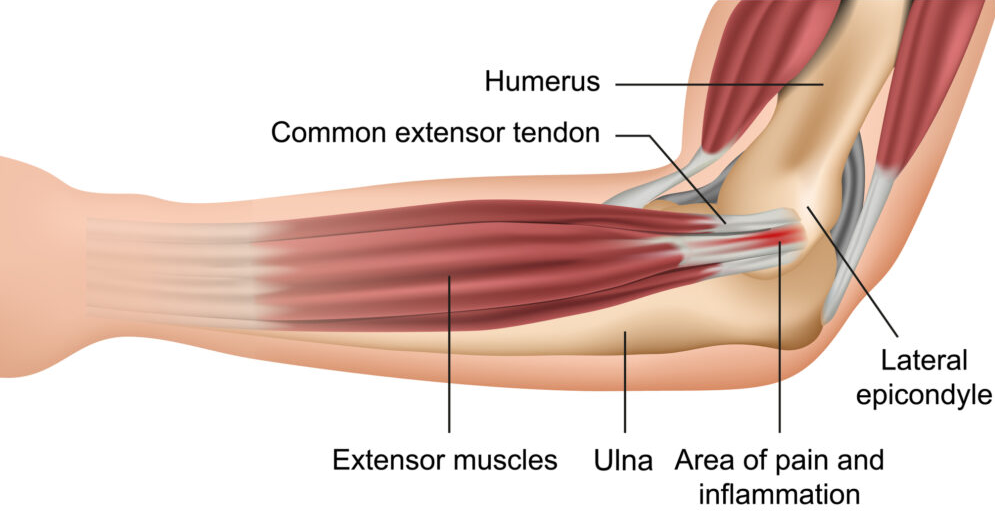
\includegraphics[width=0.8\textwidth]{bab2/ar_TennisElbow.png}
    \caption{Anatomy of tennis elbow. The area of pain and inflammation is shown in the region located around the lateral epicondyle, which is the main characteristic of this condition.}
    \label{fig:TennisElbow}
\end{figure}

Tennis elbow, often referred to as lateral epicondylitis, is a common musculoskeletal ailment marked by soreness and discomfort in the area of the elbow's common extensor origin. It is more prevalent in the dominant arm and is thought to impact 1\% to 3\% of adults annually. Though it can also happen as an acute injury (trauma to the lateral elbow), the condition is usually thought to be an overuse ailment requiring repetitive wrist extension against resistance \cite{TennisElbow1}.

Tennis elbow is characterized by pain and sensitivity in the area surrounding the lateral epicondyle, pain that gets worse as the middle finger and wrist are resisted, and elbow pain and stiffness. Repetitive forearm and hand motions, as those used in tennis, golf, and other sports, are frequently linked to the syndrome. People who perform repetitive gripping or lifting jobs at work may also experience it.

Case reports highlight the effectiveness of physiotherapy in improving joint movement and reducing pain. For example, a case series published in the Journal of Orthopaedic and Sports Physical Therapy detailed the use of dry needling as an alternative treatment for tennis elbow, resulting in significant improvements in patient-reported pain and function \cite{TennisElbow2}.

One of the training activities that can prevent the physical issue of tennis elbow is elbow flexion extension \cite{ElbowFlexionExtension}. The elbow flexion and extension movements are the two main types of movements performed by the elbow joint, which involve the movement of the forearm against the upper arm. Elbow flexion is the movement of bending the elbow so that the forearm comes closer to the upper arm. This movement involves muscles such as the biceps brachii, brachialis, and brachioradialis. Examples of this movement are when individuals bring their hands towards their shoulders or lift weights by bending their elbows. The elbow extension is the movement of straightening the elbow so that the forearm moves away from the upper arm. This movement involves muscles such as the triceps brachii and anconeus. Examples of this movement are when an individual pushes something away from the body or swings the arm into a straight position after bending it.
% Salah satu aktifitas latihan yang dapat mencegah terjadinya isu fisik tennis elbow adalah elbow flexion extension \cite{ElbowFlexionExtension}. Gerakan elbow flexion dan extension adalah dua jenis gerakan utama yang dilakukan oleh sendi siku, yang melibatkan pergerakan lengan bawah terhadap lengan atas. Elbow flexion adalah gerakan menekuk siku sehingga lengan bawah mendekat ke lengan atas. Gerakan ini melibatkan otot-otot seperti biceps brachii, brachialis, dan brachioradialis. Contoh dari gerakan ini adalah saat individu membawa tangan ke arah bahu atau mengangkat beban dengan menekuk siku. Adapun elbow extension adalah gerakan meluruskan siku sehingga lengan bawah menjauh dari lengan atas. Gerakan ini melibatkan otot-otot seperti triceps brachii dan anconeus. Contoh dari gerakan ini adalah saat seorang individu mendorong sesuatu menjauh dari tubuh atau mengayunkan lengan ke posisi lurus setelah menekuknya.

\subsection{Knee Pain and Exercise Activity}
\label{KneePain}
Knee pain is a common and multifaceted condition that can be caused by various factors, including osteoarthritis, patellofemoral pain, meniscal tears, and other conditions. About 25\% of adults exprience knee discomfort, a condition that has become much more common during the previous 20 years \cite{KneePain1}. Osteoarthritis, meniscal tears, patellofemoral discomfort, quadriceps or patellar tendinopathy, pes anserine bursitis, and iliotibial band syndrome are among the common causes. Running, crouching, and ascending stairs can all aggravate pain that is localized to particular parts of the knee, such as the anterior, medial, lateral, or posterior regions. A tool for determining the location and pattern of knee pain is the Knee Pain Map, which can be useful in both diagnosing and treating knee pain \cite{KneePain2, KneePain3}.

\begin{figure}[h!]
    \centering
    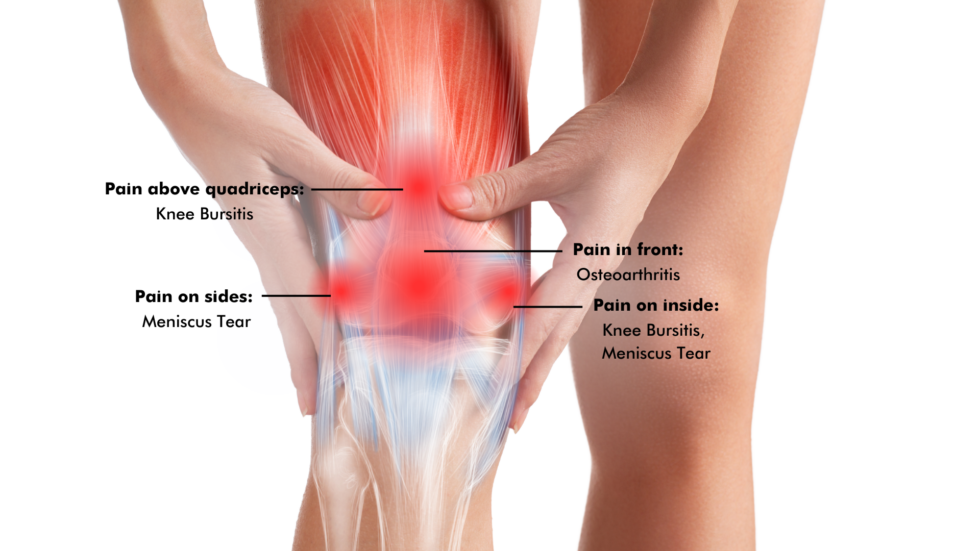
\includegraphics[width=0.9\textwidth]{bab2/ar_KneePain.png}
    \caption{Illustration of a set of issues located at the knee.}
    \label{fig:KneePain}
\end{figure}

There are two approaches in solving knee pain problems, namely exercise therapy and radiography. First-line management for osteoarthritis, patellofemoral pain, and meniscal tears often involves exercise therapy, weight loss (if overweight), education, and self-management programs to empower patients to better manage their condition \cite{KneePain4}. Radiography may be necessary to further evaluate undifferentiated knee pain, but should be reserved for chronic knee pain of more than six weeks duration or acute traumatic pain in patients who meet specific evidence-based criteria \cite{KneePain1}.

Knee pain is a frequent issue that has to be evaluated thoroughly. To confirm the diagnosis, a regular history and physical examination as well as imaging and laboratory tests may be necessary. Exercise therapy, weight loss, education, and self-management programs are common forms of treatment. In cases of severe meniscal tears or end-stage osteoarthritis, surgical referral is taken into consideration.

Exercise activities that can prevent this physical issue include leg flexion extension and knee flexion extension. Leg flexion and extension movements are the two main types of movements performed by the knee joint that involve the movement of the leg against the body. In the leg flexion stage, flexion of the knee is the movement of bending the knee so that the heel approaches the buttocks. The muscles involved in this movement include the hamstrings (biceps femoris, semitendinosus, and semimembranosus). Whereas in leg extension, extension of the knee is the movement of straightening the knee so that the leg returns to a straight position. The muscles involved include the quadriceps (rectus femoris, vastus lateralis, vastus medialis, and vastus intermedius). Leg bending and straightening movements are often performed in walking and running activities \cite{LegFlexionExtension}.
% Aktifitas-aktifitas latihan yang dapat mencegah terjadinya isu fisik ini diantaranya adalah leg flexion extension dan knee flexion extension. Gerakan leg flexion dan extension adalah dua jenis gerakan utama yang dilakukan oleh sendi lutut yang melibatkan pergerakan kaki terhadap tubuh. Pada tahap leg flexion, flexion pada lutut adalah gerakan menekuk lutut sehingga tumit mendekati bokong. Otot-otot yang terlibat dalam gerakan ini termasuk hamstrings (biceps femoris, semitendinosus, dan semimembranosus). Sedangkan pada leg extension, extension pada lutut adalah gerakan meluruskan lutut sehingga kaki kembali ke posisi lurus. Otot-otot yang terlibat termasuk quadriceps (rectus femoris, vastus lateralis, vastus medialis, dan vastus intermedius). Gerakan menekuk dan melurusan kaki sering dilakukan pada aktifitas berjalan dan berlari \cite{LegFlexionExtension}.

The knee flexion and extension movements are the two main types of movements performed by the knee joint, which involve the movement of the lower leg relative to the upper leg. In the knee flexion stage, the movement involves bending the knee so that the lower leg approaches the buttocks. The main muscles involved in this movement are the hamstrings, which consist of the biceps femoris, semitendinosus and semimembranosus. Movements that are often done daily such as squatting positions. As for knee extension, the movement that occurs is straightening the knee so that the lower leg moves away from the buttocks and returns to a straight position. The main muscles involved in this movement are the quadriceps, which consists of the rectus femoris, vastus lateralis, vastus medialis, and vastus intermedius. Daily activities that involve this movement include standing up from a squatting position \cite{KneeFlexionExtension}.
% Gerakan knee flexion dan extension adalah dua jenis gerakan utama yang dilakukan oleh sendi lutut, yang melibatkan pergerakan kaki bagian bawah terhadap kaki bagian atas. Pada tahap knee flexion, gerakan yang terjadi adalah menekuk lutut sehingga kaki bagian bawah mendekati bokong. Otot-otot utama yang terlibat dalam gerakan ini adalah hamstrings, yang terdiri dari biceps femoris, semitendinosus, dan semimembranosus. Gerakan yang sering dilakukan sehari-hari seperti posisi jongkok. Adapun knee extension, gerakan yang terjadi adalah meluruskan lutut sehingga kaki bagian bawah menjauh dari bokong dan kembali ke posisi lurus. Otot-otot utama yang terlibat dalam gerakan ini adalah quadriceps, yang terdiri dari rectus femoris, vastus lateralis, vastus medialis, dan vastus intermedius. Aktifitas sehari-hari yang melibatkan gerakan ini seperti berdiri dari posisi jongkok \cite{KneeFlexionExtension}.

\section{Human Pose Estimation}
Pose estimation is a field of computer vision research that has been widely developed for multiple purposes. Pose estimation involves detecting, associating, and tracking data points on body parts that represent the human body. Pose estimation focuses on estimating the positions of body parts using predefined keypoints. Pose estimation can also be used for tracking human activity. For instance, pose estimation from images or videos in motion is used for healthcare monitoring \cite{healthcare1,healthcare2}, sports \cite{sport1, sport2, sport3}, sign language understanding \cite{signlanguage1,signlanguage2,signlanguage3}, psychology \cite{Psychology1,Psychology2, Psychology3}, and human gesture control \cite{BlazePose, Heuristic}. Generally, human pose estimation consists of two approaches, i.e., the top-down approach and the bottom-up approach.


% Estimasi pose umumnya terdiri dari dua pendekatan, yaitu \textit{top-down} dan \textit{bottom-up}. Pendekatan \textit{top-down} dilakukan dalam dua tahap. Metode ini dimulai dengan pendeteksian orang, yang kemudian diikuti dengan penentuan pose mereka. Pendekatan ini membutuhkan komputasi yang banyak ketika jumlah orang yang terdeteksi dalam suatu \textit{frame} meningkat. High-Resolution Net (HRNet) \cite{HRNet} dan Mask R-CNN \cite{MaskRCNN} adalah beberapa model yang menggunakan pendekatan ini. Sebaliknya, pendekatan \textit{bottom-up} mendeteksi setiap sendi tubuh \textit{(keypoint)}, yang kemudian berkembang menjadi individu-tunggal. Metode ini memperkirakan probabilitas bahwa suatu sendi \textit{(keypoint)} tertentu akan hadir di piksel mana pun menggunakan peta probabilitas yang disebut \textit{heatmaps}. Pendekatan ini cukup sensitif terhadap jumlah orang dan resolusi gambar input. Berbagai penelitian terbaru telah meningkatkan pendekatan \textit{bottom-up}. Masalah pose manusia dalam resolusi gambar tertentu telah diusulkan dalam \cite{Openpose}.

\subsection{Top-Down Approach}
This method detects the persons first then the landmarks are localized for each person. The localization aims to determine the keypoints. An increase in the number of people indicates a higher level of computational complexity. They perform well on popular benchmarks in terms of accuracy. However, due to the complexity of these models, achieving real-time inference is computationally expensive \cite{YOLO-Pose}. The majority of top-down techniques now in use make use of human detector models like High-Resolution Net (HRNet) \cite{HRNet}, AlphaPose \cite{AlphaPose}, Feature Pyramid Networks \cite{Feature_Pyramid_Network}, Faster R-CNN \cite{FasterRCNN}, and Mask R-CNN \cite{MaskRCNN}. One of the first top-down models to use the Faster R-CNN for the person detection step is proposed by Papandreou et al. \cite{Papandreou}. The Cascaded Pyramid Network (CPN), developed by Chen et al. \cite{Cascade}, which integrates multi-scale feature maps from various GlobalNet layers with an online hard keypoint mining loss for challenging-to-detect joints.

\begin{figure}[h!]
    \centering
    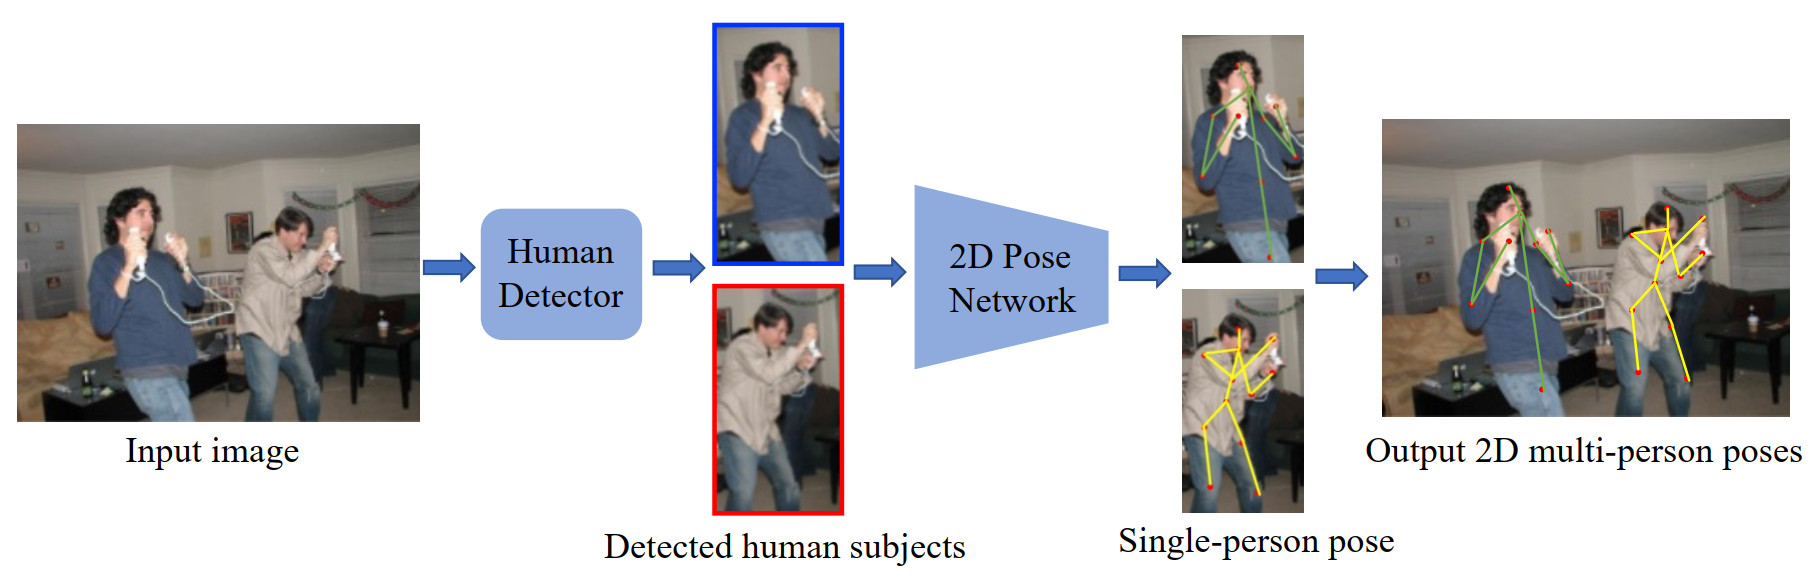
\includegraphics[width=0.9\textwidth]{bab2/ar_TopDown.png}
    \caption{Illustration of top-down approach in a 2D human pose estimation task \cite{HPEApproaches}.}
    \label{fig:TopDown}
\end{figure}

Figure \ref{fig:TopDown} shows an example of a top-down approach in human pose estimation. The process begins with an input image containing one or more people. The input image is then processed by a human detector that detects the presence of human subjects in the image. This human detector marks a bounding box around each detected individual. Once detected, the human subject is clearly identified within a bounding box. Then each individual in the image is processed in a separate state. One example of the model used is the 2D pose network. Each bounding box containing an individual is then fed into a 2D pose network. This network is responsible for estimating human poses so as to produce body keypoint coordinates for each detected subject. The resulting keypoints may vary depending on the deep learning model used. The result of this estimation is the pose of the individual in the form of keypoints connected by lines that indicate the basic skeletal of the body. After each individual has been estimated, the separate images are then reassembled according to the input image. This final image shows the pose estimation results together.
% Gambar \ref{fig:TopDown} menunjukkan contoh pendekatan top-down dalam estimasi pose manusia. Proses diawali dengan gambar input yang berisi satu atau lebih orang. Gambar input kemudian diproses oleh detektor manusia yang mendeteksi keberadaan subjek manusia dalam gambar. Detektor manusia ini menandai bounding box di sekitar setiap individu yang terdeteksi. Setelah terdeteksi, subjek manusia diidentifikasi dengan jelas dalam sebuah bounding box. Kemudian setiap individu dalam gambar diproses dalam kondisi terpisah. Salah satu contoh model yang digunakan adalah 2D pose network. Setiap bounding box yang berisikan individu ini kemudian dimasukkan ke dalam 2D pose network. Jaringan inilah yang bertanggung jawab dalam mengestimasi pose manusia sehingga menghasilkan koordinat keypoint tubuh untuk setiap subjek yang terdeteksi. Keypoint yang dihasilkan dapat berbeda-beda, bergantung pada model deep learning yang digunakan. Hasil dari estimasi ini adalah pose individu dalam bentuk keypoint yang terhubung oleh garis-garis yang menunjukkan skeletal dasar dari tubuh. Setelah setiap individu terestimasi, setiap gambar yang terpisah tadi kemudian disatukan kembali sesuai dengan gambar input. Gambar akhir ini menunjukkan hasil estimasi pose secara bersamaan.

\subsection{Bottom-Up Approach}
In this approach, it finds keypoints of all the persons in an image at once, followed by grouping them into individual persons \cite{bottom-up}. A probabilistic map called heatmap is used by these approaches to estimate the probability of every pixel containing a particular landmark (keypoint). With the help of Non-Maximum Suppression, the best landmark is filtered. These are less complex compared to Top-down methods but at the cost of reduced accuracy \cite{YOLO-Pose}. The method adopted to group recognized body parts in a picture is where different techniques diverge. Some examples of these approach models are OpenPose \cite{Openpose}, PifPaf \cite{PifPaf}, and single-stage encoder-decoder \cite{Nimbro}. To forecast keypoint heatmaps and part affinity fields, which are 2D vectors describing the relationships between joints, OpenPose \cite{Openpose} creates a model with two branches. In the grouping procedure, an affinity field is employed in part. Using the embedding spaces, Pose Partition Networks \cite{PosePartitionNetwork} propose a dense regression method across all the keypoints to construct individual partitions.

\begin{figure}[h!]
    \centering
    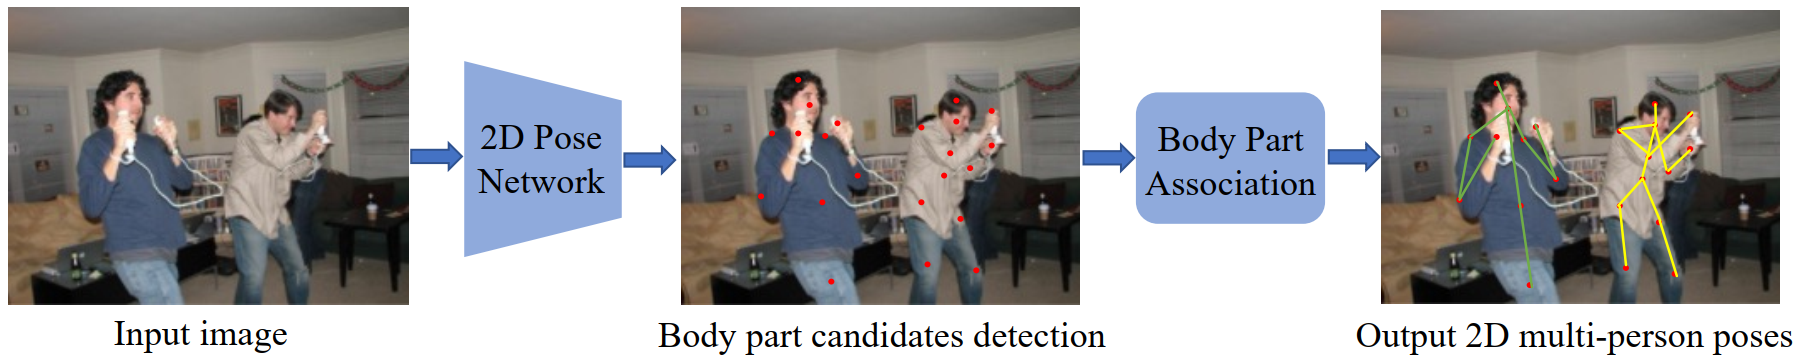
\includegraphics[width=0.9\textwidth]{bab2/ar_BottomUp.png}
    \caption{Illustration of top-down approach in a 2D human pose estimation task \cite{HPEApproaches}.}
    \label{fig:BottomUp}
\end{figure}

Figure \ref{fig:BottomUp} shows an example of a bottom-up approach in human pose estimation. For example, the model used in this estimation is a 2D pose network. The process starts with an input image containing single or multiple individuals. This input image is processed by the 2D pose network. This network is responsible for detecting possible humans in the input image. In the detection process, the network will first detect human body candidates. These points indicate the possible locations of certain body parts depending on the keypoints specified by the model. The next process is human body association. Each of these points will be connected to each other to form the skeleton of a human pose. This process matches the detected body parts into the human skeletal structure of each person in the image. The end of this approach is a multi-person pose. The result is the complete pose of each person in the image, displayed with keypoints connected by lines indicating the skeletal structure.
% Gambar \ref{fig:BottomUp} menunjukkan contoh pendekatan bottom-up dalam estimasi pose manusia. Sebagai contoh, model yang digunakan pada estimasi ini adalah 2D pose network. Proses diawali dengan sebuah gambar input yang berisikan dengan individu tunggal maupun multi. Gambar input ini diproses oleh 2D pose network. Jaringan inilah yang bertanggun jawab dalam mendeteksi kemungkinan-kemungkinan manusia yang berada di dalam gambar input. Dalam proses deteksinya, jaringan akan mendeteksi kandidat-kandidat tubuh manusia terlebih dahulu. Titik-titik ini menunjukkan kemungkinan lokasi bagian tubuh tertentu bergantung pada keypoint yang ditentukan oleh model. Proses berikutnya adalah asosiasi tubuh manusia. Setiap titik-titik ini akan dihubungkan satu sama lain membentuk kerangka pose manusia. Proses ini mencocokkan bagian tubuh yang terdeteksi ke dalam struktur kerangka manusia setiap orangnya dalam gambar. Akhir dari pendekatan ini adalah pose untul multi-orang. Hasilnya adalah pose lengkap dari setiap orang dalam gambar, ditampilkan dengan keypoint yang terhubung oleh garis yang menunjukkan struktur skeletal.

\section{MediaPipe Pose Estimation}
One of the frameworks for human pose estimation is Mediapipe Pose Estimation (MPE). MPE is an open-source cross-platform framework provided by Google for estimating 2D human joint coordinates in each image frame \cite{MPE}. MPE builds pipelines that analyzes cognitive data provided as video using machine learning (ML).

\begin{figure}[H]
    \centering
    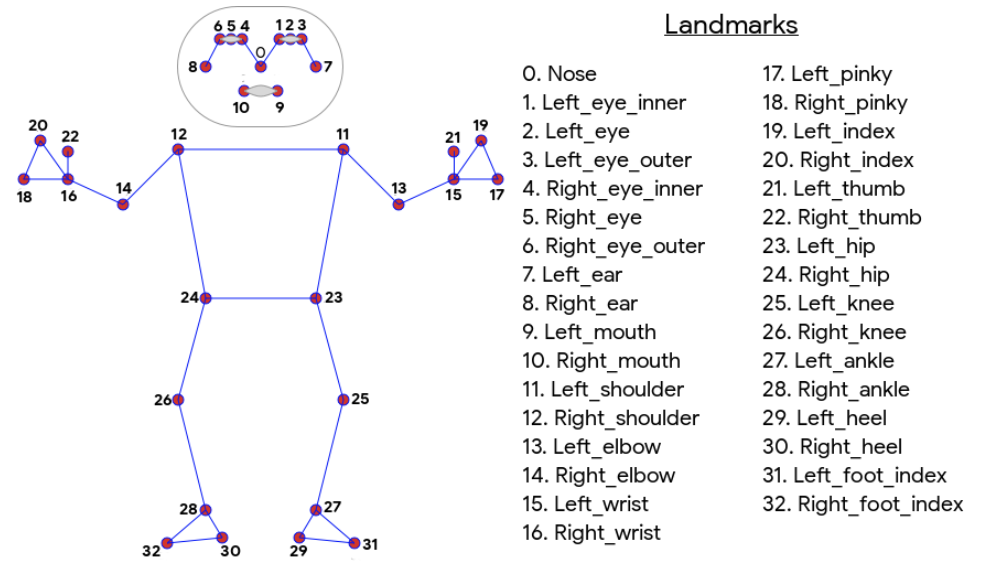
\includegraphics[width=1\textwidth]{bab2/ar_BlazePoseKeypointTopology.png}
    \caption{BlazePose keypoint topology.}
    \label{fig:BlazePoseKeypointTopology}
\end{figure}

The backbone architecture behind this framework is called BlazePose \cite{BlazePose}. Fig.\ref{fig:InferencePipeline} shows the inference workflow of BlazePose architecture. The pose estimate component of BlazePose architecture predicts the location of all 33 person keypoints. During inference, the architecture adopt a detector-tracker configuration, which displays good real-time performance on a range of applications such as hand landmark prediction \cite{MediaPipeHands} and dense face landmark prediction \cite{MediaPipeDenseFace}. This pipeline comprises of a lightweight body pose detector followed by a pose tracker network. The tracker predicts keypoint coordinates, the presence of the person on the current frame, and the refined region of interest for the current frame. When the tracker reports that there is no human present, the architecture re-run the detection network on the following frame.

Pose estimation using the BlazePose architecture offers the advantage of producing lightweight models. For low-computational devices, a lightweight model is highly preferred. BlazePose is a lightweight convolutional architecture designed for real-time pose estimation. On a single mid-tier phone CPU, the frame rate for the BlazePose Full architecture is 10 FPS while the BlazePose Lite architecture is 31 FPS \cite{BlazeFace}.

\begin{figure}[h!]
    \centering
    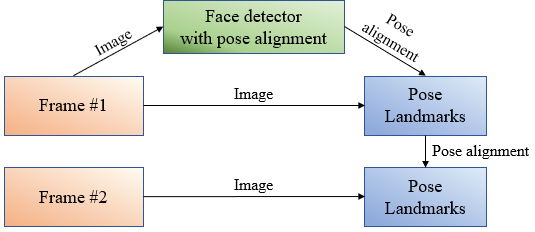
\includegraphics[width=0.75\textwidth]{bab2/ar_InferencePipeline.png}
    \caption{Inference workflow of BlazePose architecture \cite{BlazePose}.}
    \label{fig:InferencePipeline}
\end{figure}

\section{Deep Learning}
\label{sec2:DeepLearning}

Deep learning is a branch of machine learning that uses artificial neural networks to analyze and extract patterns from large and complex data. Artificial neural networks, which are composed of linked layers of artificial neurons, including input layers, hidden layers, and output layers, are computer models that are modeled after the structure and operation of the human brain. The utilization of numerous hidden layers, which enables the model to learn increasingly complicated data representations, is one of the primary features of deep learning \cite{DL3}.

Deep learning is particularly effective when used on large and diverse datasets, allowing the model to improve accuracy and performance. The learning process in deep learning involves optimizing model parameters using algorithms such as stochastic gradient descent (SGD) and backpropagation techniques to update the weights in the neural network based on the error gradient, allowing the network to learn from errors.

\begin{figure}[H]
    \centering
    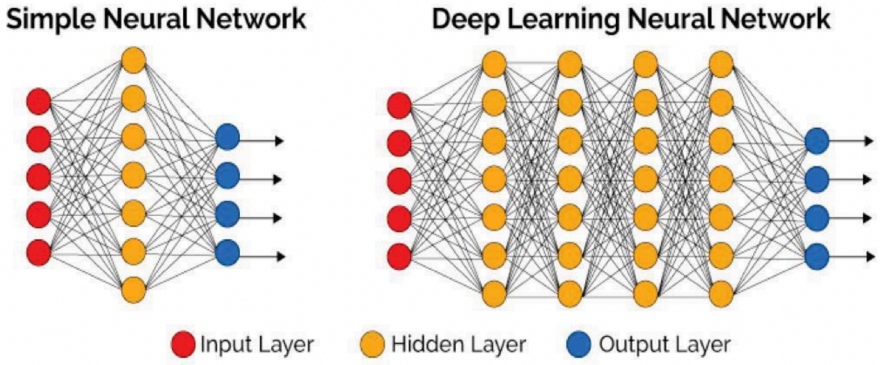
\includegraphics[width=0.9\textwidth]{bab2/ar_DLArchitecture.png}
    \caption{Compared between simple neural network architecture and deep learning neural network.}
    \label{fig:DLArchitecture}
\end{figure}

Deep Learning is a type of machine learning that excels in working with unstructured data. It has the capability to process a huge number of characteristics \cite{DL1}. Deep Learning algorithms process data over numerous levels. Each layer in Deep Learning increasingly extracts features and transmits them to the next layer. The early layers in Deep Learning are responsible for extracting low-level information, while subsequent layers combine various features to build a full representation. Deep Learning is connected to artificial neural networks, which are algorithms based on the structure and function of the brain.

Deep Learning enables computational models with several layers of processing to learn various degrees of abstraction for data representation. The layers in Deep Learning are neural networks with more than three layers of neurons (including input and output layers). More layers and neurons can represent increasingly complicated models, but they also require more time and resources for processing. The depiction of the Deep Learning architecture is presented in Figure \ref{fig:DLArchitecture} \cite{DL2}.

Types of deep learning networks include Convolutional Neural Networks (CNN) used in image and video processing, Recurrent Neural Networks (RNN) suitable for sequential data such as text and audio, and Generative Adversarial Networks (GAN) used for data generation. Applications of deep learning include image and speech recognition, natural language processing (NLP), autonomous vehicles, medical data analysis, and recommendation systems.

Deep learning has revolutionized many fields with the ability to learn and generalize from complex and unstructured data, enabling the development of advanced technologies such as virtual assistants and automated medical diagnosis.

\subsection{Convolutional Neural Network (CNN)}
CNN (Convolutional Neural Network) has applications in image and video recognition, recommendation systems, image classification, medical image analysis, natural language processing, and financial time series analysis. Traditional neural network methods do not perform well when it comes to image processing and need breaking down pictures into low-resolution patches. CNN has neurons arranged as portions involved for processing visual input in humans and other. The layers of neurons are designed in such a manner that they span the full visual field to avoid the gradual image processing difficulties of typical neural networks. The sequence of CNN layers includes of input layers, output layers, and hidden layers that contain numerous convolutional layers, pooling layers, and fully connected layers, as depicted in Figure \ref{fig:CNNArchitecture} \cite{CNN1}.

\begin{figure}[H]
    \centering
    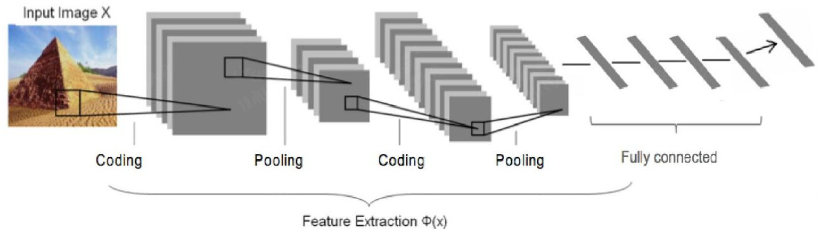
\includegraphics[width=1\textwidth]{bab2/ar_CNNArchitecture.png}
    \caption{An example of CNN architecture for image recognition \cite{cnnarch}.}
    \label{fig:CNNArchitecture}
\end{figure}

Convolution operation is a crucial component of convolutional neural networks. The convolutional layer consists of parameters that comprise a set of learnable filters (kernels). Each filter in this layer is small in width and height but extends through the full depth of the input volume. The commonly used filter sizes are 3x3, 5x5, and 7x7. The third dimension of the filter corresponds to the number of channels in the input. The depth of a grayscale image is 1, while a color image has 3 color channels (RGB).

CNN often employs pooling layers after the convolutional layers. These layers serve to lower the dimensions, often known as subsampling or downsampling. The hyperparameters of the pooling layer are the filter size and stride. The most typically used pooling layer has a filter size of 2 and a stride of 2. There are two main forms of pooling: max pooling, which takes the maximum value, and average pooling, which takes the average value. Max pooling is more often utilized than average pooling.

After several convolutional and pooling layers, CNN typically ends with several fully connected layers. The tensors from the output of these layers are flattened into vectors and then passed through several neural network layers. The dropout regularization technique can be applied to the fully connected layers to prevent overfitting. The final fully connected layer in the architecture contains the same number of output neurons as the number of classes to be recognized in an object detection model.

\subsection{Long Short-Term Memory (LSTM)}
LSTM network is an enhanced special network architecture of Recurrent Neural Network (RNN) \cite{RNN} which has its major usage in evaluating time series data of many disciplines. LSTM was meant to reduce the drawbacks of RNN such as vanishing gradient because of having short term memory. LSTM is capable of modeling the time series sequential data. A memory unit known as the cell was introduced in the network. As a result, LSTM can overcome the long-range dependency issue of RNN as it can keep the findings for a long-range of time \cite{LSTM1}.

\begin{figure}[H]
    \centering
    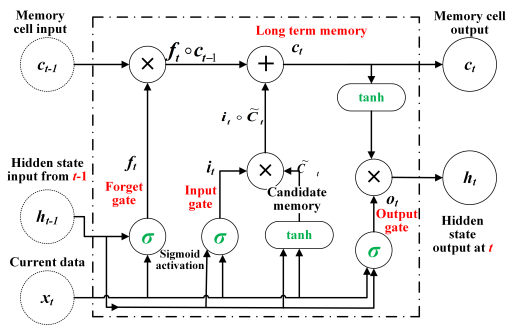
\includegraphics[width=0.75\textwidth]{bab2/ar_OneCellLSTM.png}
    \caption{Illustration of one cell of the LSTM memory block.}
    \label{fig:OneCellLSTM}
\end{figure}

The fundamental LSTM unit is shown in Fig. \ref{fig:OneCellLSTM}, and is made of a cell with an input gate, output gate, and forget gate. LSTMs use the concept of gating to deal with the disappearing or exploding gradient problem \cite{LSTM2}. The cell is responsible for remembering values over arbitrary time intervals, and each of the three gates can be thought of as a conventional artificial neuron, computing an activation (using an activation function) of a weighted sum of the current data $x_{t}$, a hidden state $h_{t-1}$ from the previous time step, and any bias $b$. Intuitively, the gates can be considered as regulators of the flow of values through the connections of the LSTM. At each time step they govern which action is done by the cell as stated below. In \ref{equ:WriteOperation} through \ref{equ:Output}, $w_{i}$ are the weights associated with each multiplication at gate $i$, while $\sigma$ and $tanh$ are possibilities for the activation functions.

Based on Fig. \ref{fig:OneCellLSTM}, the output gate controls the amount to which a new value flows into the cell, known as a write operation:
\begin{equation}
    \label{equ:WriteOperation}
    i_t=\sigma(w_i[h_{t-1},x_t]+b_i)
\end{equation}

The forget gate performs a similar process, regulating the amount to which the current cell value is preserved, executing a reset operation
\begin{equation}
    \label{equ:ResetOperation}
    f_t=\sigma(w_f[h_{t-1},x_t]+b_f)
\end{equation}

The candidate memory cell is updated similarly as:
\begin{equation}
    \label{equ:NewCandidateValue}
    \tilde{C}_t=\tanh(w_c[h_{t-1},x_t]+b_c)
\end{equation}

and by merging these distinct internal values the internal long-term memory or the next cell memory is formed as
\begin{equation}
    \label{equ:Combination}
    c_t=f_t*c_t+i_t*\tilde{C}_t
\end{equation}

From this, the cell output is created by the output gate to regulate the extent to which the value in the cell is utilized to compute the output activation, conducting a read operation:
\begin{equation}
    \label{equ:ReadOperation}
    o_t=\sigma(w_o[h_{t-1},x_t]+b_o)
\end{equation}

Lasltly, the cell's hidden output is found as
\begin{equation}
    \label{equ:Output}
    h_t=o_t*\tanh(c_t)
\end{equation}

\section{Performance Metrics}
\label{sec3: performance_metrics}

Performance metrics in deep learning are measures used to evaluate model performance. They offer information on how well the model can forecast new and never-before-seen data. Large datasets are frequently used to train models in deep learning, and performance metrics are used to evaluate the model's performance under various conditions. Here are some commonly used performance metrics in deep learning.

\subsection{Confusion Matrix}
\label{subsec3: confusion_matrix}
The confusion matrix is a tool used to measure the performance of a classification model by providing a detailed overview of the model's predictions against the test data. It is a box-shaped matrix that shows the number of correct and incorrect predictions made by the model. The number of predictions is based on the actual class and the predicted class. Figure A shows the elements in the confusion matrix, namely True Positive (TP), True Negative (TN), False Positive (FP), and False Negative (FP). Through this matrix, various performance metrics can be measured, such as precision, recall, accuracy, and loss.
% Confusion matrix adalah alat yang digunakan untuk mengukur kinerja model klasifikasi dengan memberikan gambaran rinci tentang hasil prediksi model terhadap data uji. Matriks ini berbentuk kotak yang memperlihatkan jumlah prediksi benar dan salah yang dibuat oleh model. Jumlah prediksi tersebut didasarkan kepada kelas yang sebenarnya dengan kelas yang diprediksi. Gambar A menunjukkan elemen-elemen di dalam confusion matrix, yaitu True Positive (TP), True Negative (TN), False Positive (FP), dan False Negative (FP). Melalui matrix ini, berbagai peforma metric dapat diukur, seperti  presisi, recall, akurasi, dan loss.

\begin{figure}[h!]
    \centering
    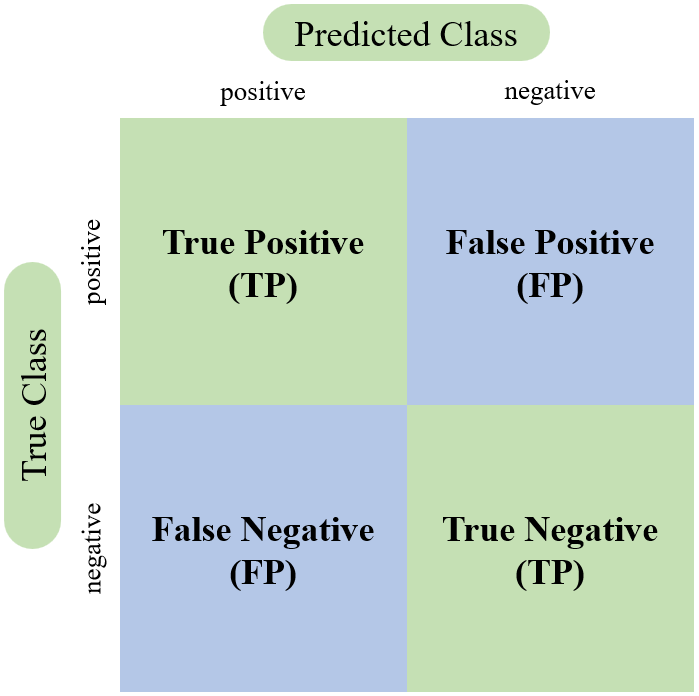
\includegraphics[width=0.5\textwidth]{bab2/ar_confmatrix.png}
    \caption{A common example of a confusion matrix.}
    \label{fig: convmatrix}
\end{figure}

\subsection{Accuracy}
\label{subsec3: accuracy}

\begin{figure}[h!]
    \centering
    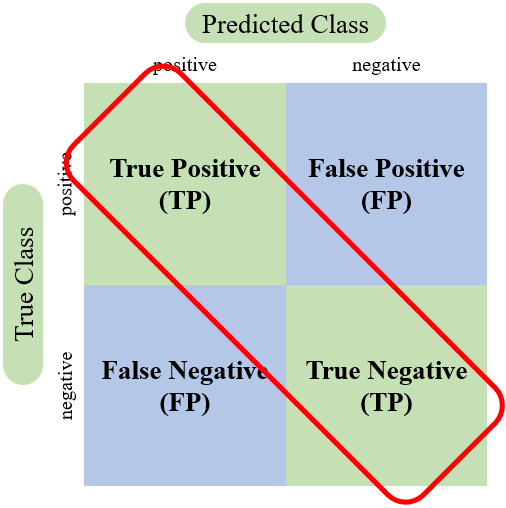
\includegraphics[width=0.5\textwidth]{bab2/ar_Accuracy.png}
    \caption{Accuracy is calculated as the ratio of the number of correct predictions to the total number of predictions.}
    \label{fig:MetricAccuracy}
\end{figure}

Accuracy is an evaluation measure used to assess model performance by calculating the proportion of correct predictions to total predictions. Accuracy shows how well the model performs overall. The accuracy equation is directly proportional to the True Positive (TP) and inversely proportional to the total prediction samples as shown in equation \ref{equ:accuracy}.
% Akurasi merupakan ukuran evaluasi yang digunakan untuk menilai kinerja model dengan menghitung proporsi prediksi yang benar terhadap total prediksi keseluruhan. Akurasi menunjukkan seberapa baik peforma model secara keseluruhan. Persamaan akurasi berbanding lurus dengan True Positive (TP) dan berbanding terbalik dengan total sampel prediksi sebagaimana ditunjukkan pada persamaan \ref{equ:accuracy}.

\begin{equation}
    \label{equ:accuracy}
    accuracy=\frac{TP+TN}{TP+TN+FP+FN}
\end{equation}

\subsection{Loss}
\label{equ:loss}
Loss is a function used to calculate the error of the deep learning model during the learning process. It is a quantitative measure that describes how well or poorly the model predicts the class of the input data compared to the ground truth. This function gives an indication of how far the model's prediction is from the correct value with the aim of minimizing the loss value during the training process to improve the accuracy and overall performance of the model.
% Loss merupakan fungsi yang digunakan untuk menghitung kesalahan model deep learning selama proses learning. Metris ini adalah ukuran kuantitatif yang menggambarkan seberapa baik maupun buruk model dalam memprediksi kelas dari data input dibandingkan dengan groun truth. Fungsi ini memberikan indikasi seberapa jauh prediksi model dari nilai yang benar dengan tujuan meminimalkan nilai loss selama proses pelatihan untuk meningkatkan akurasi dan kinerja model secara keseluruhan.

\subsection{Precision}
\label{subsec3: precision}

\begin{figure}[h!]
    \centering
    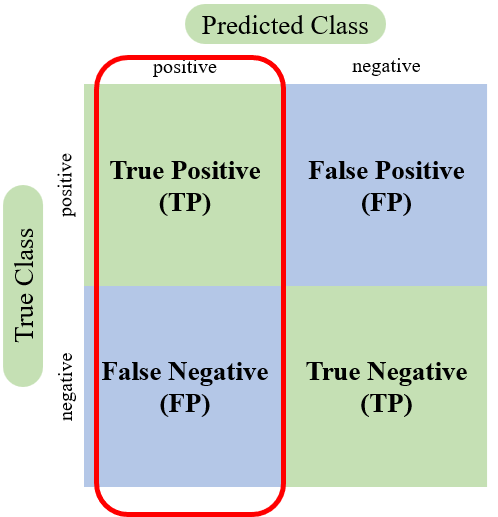
\includegraphics[width=0.5\textwidth]{bab2/ar_Precision.png}
    \caption{Precision is calculated as the ratio of the number of correct positive predictions to the total number of positive predictions made by the model.}
    \label{fig:MetricPrecision}
\end{figure}

Precision is a metrics that measures the proportion of correct positive predictions out of all predictions. Precision measures how well the model can find True Positive (TP) out of all positive predictions (TP+FP). The higher the precision value, the more positive predictions are predicted to be true. This metric becomes very important when in a situation where the false positive value is high. Precision is formulated in the equation \ref{equ:precision}.
% Precision adalah metrics yang mengukur proporsi prediksi positif yang benar dari semua prediksi. Precision mengukur seberapa baik model dapat menemukan True Positive (TP) dari semua prediksi positif (TP+FP). Semakin tinggi nilai precision menunjukkan semakin banyak prediksi positif yang diprediksi benar. Metric ini menjadi sangat penting ketika berada dalam situasi di mana nilai false positive tinggi. Precision dirumuskan pada persamaan \ref{equ:precision}. 

\begin{equation}
    \label{equ:precision}
    precision=\frac{TP}{TP+FP}
\end{equation}

\subsection{Recall}
\label{subsec3: recall}

\begin{figure}[h!]
    \centering
    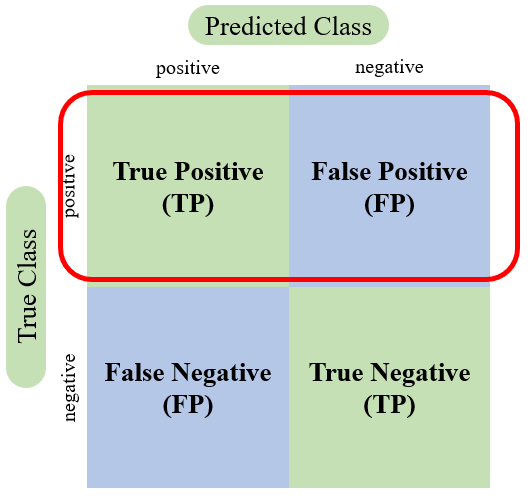
\includegraphics[width=0.5\textwidth]{bab2/ar_Recall.png}
    \caption{Recall is calculated as the ratio of the number of correct positive predictions to the total number of positive examples actually present in the dataset.}
    \label{fig:MetricRecall}
\end{figure}

This metric is used to measure how well the model can detect all positive events among all events that are actually positive. This metric becomes very important when false negatives have a significant probability. Recall is calculated as True Positive (TP) divided by the sum of True Positive and False Negative (TP+FN), according to the equation \ref{equ:recall}.
% Metric ini digunakan untuk mengukur seberapa baik model dapat mendeteksi seluruh kejadian positif di antara seluruh kejadian yang sebenarnya positif. Metric ini menjadi sangat penting ketika false negative memiliki kemungkinan yang signifikan. Recall dihitung sebagai True Positive (TP) dibagi dengan jumlah True Positive dan False Negative (TP+FN), sesuai dengan persamaan \ref{equ:recall}.

\begin{equation}
    \label{equ:recall}
    recall=\frac{TP}{TP+FN}
\end{equation}

\subsection{F1-Score}
\label{subsec3: f1score}
Another metric used is F1 score. The F1 score is a metric commonly used to measure the performance of a classification model. It is the harmonic mean of precision and recall. The F1 score combines precision and recall into a single value, providing a balanced measure of the model's performance. It is calculated using the following equation \ref{equ:f1score}.

\begin{equation}
    \label{equ:f1score}
    F1 score = 2 * \frac{precision * recall}{precision + recall}
\end{equation}
